\documentclass[10pt,a4paper]{article}
\usepackage[margin=1.2cm]{geometry}
\usepackage{amsmath, amssymb, amsthm}
\usepackage{tikz}
\usetikzlibrary{arrows.meta, decorations.pathreplacing, calc, patterns}
\usepackage{pgfplots}
\pgfplotsset{compat=1.18}
\usepackage{mdframed}
\usepackage{xcolor}
\usepackage{enumitem}
\usepackage{titlesec}
\usepackage{booktabs}
\usepackage{array}
\usepackage{multicol}
\usepackage{caption}

% Colors
\definecolor{darkgreen}{RGB}{0,100,60}
\definecolor{teal}{RGB}{0,128,128}
\definecolor{lightbg}{RGB}{240,255,248}
\definecolor{propbg}{RGB}{230,245,255}
\definecolor{exbg}{RGB}{255,248,230}
\definecolor{headcolor}{RGB}{0,80,50}
\definecolor{stepcolor}{RGB}{0,60,120}
\definecolor{stepbg}{RGB}{235,242,255}
\definecolor{rampcolor}{RGB}{100,0,100}
\definecolor{rampbg}{RGB}{248,235,255}
\definecolor{signumbg}{RGB}{255,240,235}
\definecolor{rectbg}{RGB}{240,255,240}
\definecolor{expbg}{RGB}{255,252,235}
\definecolor{notebg}{RGB}{255,245,245}
\definecolor{notecolor}{RGB}{150,0,0}
\definecolor{intuitbg}{RGB}{245,245,255}
\definecolor{intuitcolor}{RGB}{50,50,150}

% Section formatting
\titleformat{\section}{\large\bfseries\color{headcolor}}{}{0em}{}[\titlerule]
\titleformat{\subsection}{\normalsize\bfseries\color{darkgreen}}{}{0em}{}
\titleformat{\subsubsection}{\small\bfseries\color{stepcolor}}{}{0em}{}
\titlespacing{\section}{0pt}{8pt}{3pt}
\titlespacing{\subsection}{0pt}{5pt}{2pt}
\titlespacing{\subsubsection}{0pt}{4pt}{1pt}

% Box environments
\newmdenv[backgroundcolor=lightbg, linecolor=darkgreen, linewidth=1pt,
  innertopmargin=4pt, innerbottommargin=4pt, innerleftmargin=6pt,
  innerrightmargin=6pt, skipabove=3pt, skipbelow=3pt]{defbox}
\newmdenv[backgroundcolor=propbg, linecolor=teal, linewidth=1pt,
  innertopmargin=4pt, innerbottommargin=4pt, innerleftmargin=6pt,
  innerrightmargin=6pt, skipabove=3pt, skipbelow=3pt]{propbox}
\newmdenv[backgroundcolor=exbg, linecolor=orange!70!black, linewidth=1pt,
  innertopmargin=4pt, innerbottommargin=4pt, innerleftmargin=6pt,
  innerrightmargin=6pt, skipabove=3pt, skipbelow=3pt]{exbox}
\newmdenv[backgroundcolor=stepbg, linecolor=stepcolor, linewidth=1.5pt,
  innertopmargin=5pt, innerbottommargin=5pt, innerleftmargin=6pt,
  innerrightmargin=6pt, skipabove=4pt, skipbelow=4pt]{stepbox}
\newmdenv[backgroundcolor=rampbg, linecolor=rampcolor, linewidth=1.5pt,
  innertopmargin=5pt, innerbottommargin=5pt, innerleftmargin=6pt,
  innerrightmargin=6pt, skipabove=4pt, skipbelow=4pt]{rampbox}
\newmdenv[backgroundcolor=signumbg, linecolor=red!60!black, linewidth=1.5pt,
  innertopmargin=5pt, innerbottommargin=5pt, innerleftmargin=6pt,
  innerrightmargin=6pt, skipabove=4pt, skipbelow=4pt]{signumbox}
\newmdenv[backgroundcolor=rectbg, linecolor=darkgreen!80!black, linewidth=1.5pt,
  innertopmargin=5pt, innerbottommargin=5pt, innerleftmargin=6pt,
  innerrightmargin=6pt, skipabove=4pt, skipbelow=4pt]{rectbox}
\newmdenv[backgroundcolor=expbg, linecolor=orange!60!black, linewidth=1.5pt,
  innertopmargin=5pt, innerbottommargin=5pt, innerleftmargin=6pt,
  innerrightmargin=6pt, skipabove=4pt, skipbelow=4pt]{expbox2}
\newmdenv[backgroundcolor=notebg, linecolor=notecolor, linewidth=1.2pt,
  innertopmargin=4pt, innerbottommargin=4pt, innerleftmargin=6pt,
  innerrightmargin=6pt, skipabove=3pt, skipbelow=3pt]{notebox}
\newmdenv[backgroundcolor=intuitbg, linecolor=intuitcolor, linewidth=1pt,
  innertopmargin=4pt, innerbottommargin=4pt, innerleftmargin=6pt,
  innerrightmargin=6pt, skipabove=3pt, skipbelow=3pt]{intuitbox}

\setlength{\parindent}{0pt}
\setlength{\parskip}{2pt}
\setlist[itemize]{noitemsep, topsep=1pt, leftmargin=12pt}

\begin{document}

\begin{center}
  {\LARGE\bfseries\color{headcolor} Signals \& Systems --- Comprehensive Reference}\\[3pt]
  {\small Unit Impulse $\cdot$ Sampling Property $\cdot$ Unit Step $\cdot$ Impulse--Step Relation
    $\cdot$ Unit Ramp $\cdot$ Unit Parabolic $\cdot$ Signum $\cdot$ Rectangular $\cdot$ Triangular
    $\cdot$ Sinc $\cdot$ Exponential}\\[2pt]
  {\footnotesize\color{gray} Complete treatment with derivations, properties, graphs, and solved problems}
\end{center}
\vspace{2pt}\hrule height 1.5pt\vspace{4pt}

%=============================================================
\section{1.\ Unit Impulse Signal (Dirac Delta Function)}
%=============================================================

\subsection*{1.1 Definition and Physical Motivation}

\begin{defbox}
The \textbf{Unit Impulse signal}, also called the \textbf{Dirac Delta function} $\delta(t)$, is defined as:
\[
\delta(t) = \begin{cases} \infty & t=0 \\ 0 & t\neq0 \end{cases}
\qquad\text{subject to}\qquad
\int_{-\infty}^{\infty}\delta(t)\,dt = 1 \quad\text{(area = 1, always)}
\]
The impulse is \emph{not} a conventional function; it is a \textbf{distribution} (generalized function). Its defining property is the combination of zero duration, infinite amplitude, and \textbf{unit area}.
\end{defbox}

\begin{intuitbox}
\textbf{Physical Intuition:} Imagine applying a very large force over a very short time (e.g., hitting a ball with a bat). As the contact time $\to 0$ but the impulse (force $\times$ time) is kept constant at 1, we get $\delta(t)$. Similarly, a very short, powerful voltage spike in circuits can be modeled as $\delta(t)$. The important quantity is not the instantaneous magnitude, but rather the \textit{area} (net effect) which remains exactly 1.
\end{intuitbox}

\subsection*{1.2 Graph of $\delta(t)$}

The impulse is represented by a vertical arrow at $t=0$ with the label ``$(1)$'' indicating unit area. The height is technically $\infty$ but the arrow convention encodes the weight.

\begin{center}
\begin{tikzpicture}[scale=0.9]
  \draw[->] (-2.5,0) -- (2.8,0) node[right] {$t$};
  \draw[->] (0,-0.2) -- (0,1.8) node[above] {$\delta(t)$};
  \draw[->, very thick, darkgreen] (0,0) -- (0,1.5);
  \node[below right, font=\small] at (0.05,0) {$0$};
  \node[left, font=\small] at (0,1.5) {$\infty$};
  \node[above right, font=\small, darkgreen] at (0.05,1.5) {$(1)$};
  % Zero labels on axis
  \foreach \x in {-2,-1,1,2}{
    \draw (\x,0.05) -- (\x,-0.05) node[below,font=\tiny]{\x};
  }
  \draw[darkgreen, thick] (-2.5,0) -- (-0.01,0);
  \draw[darkgreen, thick] (0.01,0) -- (2.5,0);
\end{tikzpicture}
\hspace{1.5cm}
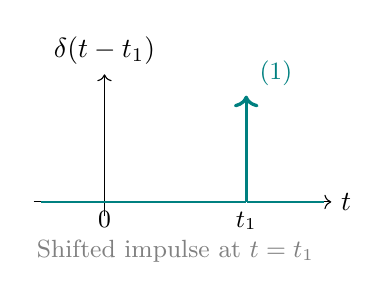
\begin{tikzpicture}[scale=0.9]
  % Shifted impulse delta(t - t1)
  \draw[->] (-1.0,0) -- (3.2,0) node[right] {$t$};
  \draw[->] (0,-0.2) -- (0,1.8) node[above] {$\delta(t-t_1)$};
  \draw[->, very thick, teal] (2,0) -- (2,1.5);
  \node[below, font=\small] at (0,0) {$0$};
  \node[below, font=\small] at (2,0) {$t_1$};
  \node[above right, font=\small, teal] at (2.05,1.5) {$(1)$};
  \draw[teal, thick] (-0.9,0) -- (1.99,0);
  \draw[teal, thick] (2.01,0) -- (3.1,0);
  \node[font=\small, color=gray] at (1.0,-0.7) {Shifted impulse at $t=t_1$};
\end{tikzpicture}
\end{center}

\subsection*{1.3 Construction via Limiting Rectangular Pulses}

The impulse can be rigorously understood as a \textbf{limit of a rectangular pulse} as its width $\to 0$ while area is preserved:

Define a rectangular pulse:
\[
x_\varepsilon(t) = \begin{cases} \dfrac{1}{\varepsilon} & -\dfrac{\varepsilon}{2} < t < \dfrac{\varepsilon}{2} \\ 0 & \text{otherwise} \end{cases}
\qquad \Rightarrow \qquad \text{Area} = \varepsilon \cdot \frac{1}{\varepsilon} = 1 \quad \forall\,\varepsilon
\]
\[
\delta(t) = \lim_{\varepsilon \to 0} x_\varepsilon(t) \qquad \Rightarrow \qquad \text{Width} \to 0,\quad \text{Height} = \frac{1}{\varepsilon} \to \infty,\quad \text{Area} = 1
\]

\begin{center}
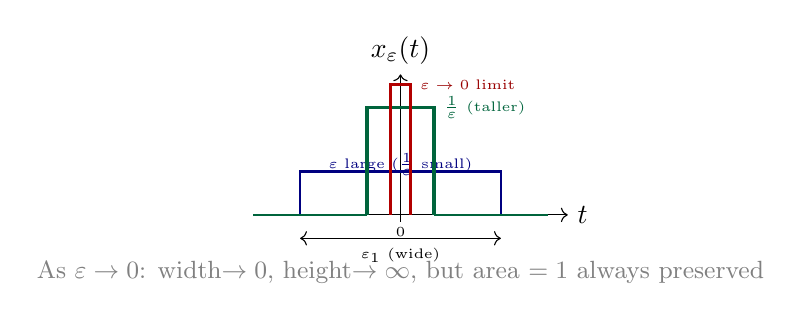
\begin{tikzpicture}[scale=0.85]
  \draw[->] (-2.2,0) -- (2.5,0) node[right] {$t$};
  \draw[->] (0,-0.1) -- (0,2.1) node[above] {$x_\varepsilon(t)$};
  % Wide pulse (large epsilon)
  \draw[blue!50!black, thick] (-1.5,0)--(-1.5,0.65)--(1.5,0.65)--(1.5,0);
  \draw[blue!50!black, thick] (-2.2,0)--(-1.5,0);
  \draw[blue!50!black, thick] (1.5,0)--(2.2,0);
  \node[blue!50!black, font=\tiny] at (0,0.75) {$\varepsilon$ large ($\frac{1}{\varepsilon}$ small)};
  \draw[<->] (-1.5,-0.35)--(1.5,-0.35) node[midway,below,font=\tiny]{$\varepsilon_1$ (wide)};
  % Narrow pulse (small epsilon)
  \draw[darkgreen, very thick] (-0.5,0)--(-0.5,1.6)--(0.5,1.6)--(0.5,0);
  \draw[darkgreen, thick] (0.5,0)--(2.2,0);
  \draw[darkgreen, thick] (-2.2,0)--(-0.5,0);
  \node[right, font=\tiny, darkgreen] at (0.5,1.6) {$\frac{1}{\varepsilon}$ (taller)};
  % Even narrower
  \draw[red!70!black, very thick] (-0.15,0)--(-0.15,1.95)--(0.15,1.95)--(0.15,0);
  \node[right, font=\tiny, red!60!black] at (0.15,1.95) {$\varepsilon\to0$ limit};
  \node[below, font=\tiny] at (0,-0.05) {$0$};
  \node[font=\small, color=gray, align=center] at (0,-0.85) {As $\varepsilon\to0$: width$\to0$, height$\to\infty$, but area $=1$ always preserved};
\end{tikzpicture}
\end{center}

\begin{notebox}
\textbf{Other limiting representations of $\delta(t)$:}
\begin{itemize}
  \item Gaussian: $\delta(t) = \lim_{\sigma\to 0} \dfrac{1}{\sigma\sqrt{2\pi}}e^{-t^2/(2\sigma^2)}$
  \item Sinc: $\delta(t) = \lim_{\omega\to\infty} \dfrac{\sin(\omega t)}{\pi t}$
  \item Triangular: $\delta(t) = \lim_{\varepsilon\to 0} \dfrac{1}{\varepsilon}\Lambda\!\left(\dfrac{t}{\varepsilon}\right)$ where $\Lambda$ is the triangular function
\end{itemize}
All share the property: finite area = 1, zero-width support, infinite peak.
\end{notebox}

\subsection*{1.4 Properties of the Unit Impulse Signal}

\begin{propbox}
\textbf{P1 --- Unit Area:}
\[
\int_{-\infty}^{\infty}\delta(t)\,dt = 1
\]
The total ``energy'' (area) of the impulse is always 1, regardless of where it is located.

\smallskip
\textbf{P2 --- Strength / Weight of Scaled Impulse:}\quad If $y(t) = A_0\,\delta(t)$, then:
\[
\int_{-\infty}^{\infty} y(t)\,dt = A_0\int_{-\infty}^{\infty}\delta(t)\,dt = A_0
\]
The coefficient $A_0$ is called the \textbf{strength} or \textbf{weight} of the impulse. Graphically, scaled impulse $A_0\,\delta(t)$ is an arrow labeled ``$(A_0)$''.

\smallskip
\textbf{P3 --- Integration gives Step:}
\[
\int_{-\infty}^{t}\delta(\tau)\,d\tau = u(t)
\qquad\text{and}\qquad
\int_{-\infty}^{t} A_0\,\delta(\tau)\,d\tau = A_0\,u(t)
\]
The running integral of the impulse equals the unit step function.

\smallskip
\textbf{P4 --- Even Symmetry:}
\[
\delta(-t) = \delta(t)
\]
The impulse is an \textbf{even function}. This follows from the rectangle approximation being symmetric about $t=0$.

\smallskip
\textbf{P5 --- Energy \& Power (NENP):}\quad Since $|\delta(0)|^2 = \infty^2$:
\[
E = \int_{-\infty}^{\infty}|\delta(t)|^2\,dt = \infty \qquad P = \lim_{T\to\infty}\frac{1}{2T}\int_{-T}^{T}|\delta(t)|^2\,dt \to \infty
\]
$E = \infty$, $P = \infty$ $\Rightarrow$ \textbf{NENP} (Neither Energy Nor Power) signal.

\smallskip
\textbf{P6 --- Time Shifting:}\quad $\delta(t) \xrightarrow{\text{T.S. by }t_1} \delta(t-t_1)$

The impulse shifts to $t = t_1$ but retains unit area:
$\displaystyle\int_{-\infty}^{\infty}\delta(t-t_1)\,dt = 1$

\begin{center}
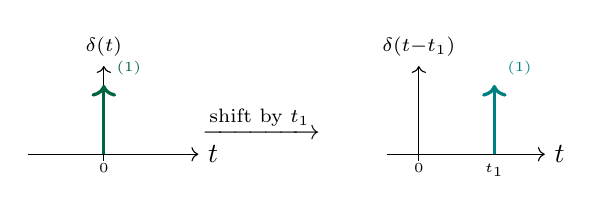
\begin{tikzpicture}[scale=0.8]
  \begin{scope}[xshift=-2.5cm]
    \draw[->](-1.2,0)--(1.5,0) node[right]{$t$};
    \draw[->](0,-0.1)--(0,1.4) node[above]{\scriptsize$\delta(t)$};
    \draw[->,very thick,darkgreen](0,0)--(0,1.1);
    \node[below,font=\tiny] at (0,0){$0$};
    \node[above right,font=\tiny,darkgreen] at (0.05,1.1){$(1)$};
  \end{scope}
  \node at(0,0.5){$\xrightarrow{\text{shift by }t_1}$};
  \begin{scope}[xshift=2.5cm]
    \draw[->](-0.5,0)--(2.0,0) node[right]{$t$};
    \draw[->](0,-0.1)--(0,1.4) node[above]{\scriptsize$\delta(t{-}t_1)$};
    \draw[->,very thick,teal](1.2,0)--(1.2,1.1);
    \node[below,font=\tiny] at(0,0){$0$};
    \node[below,font=\tiny] at(1.2,0){$t_1$};
    \node[above right,font=\tiny,teal] at(1.25,1.1){$(1)$};
  \end{scope}
\end{tikzpicture}
\end{center}

\smallskip
\textbf{P7 --- Time Scaling:}\quad For $a \neq 0$:
\[
\delta(at) = \frac{1}{|a|}\,\delta(t)
\]
\textbf{Derivation:} Use substitution $\tau = at$, so $d\tau = a\,dt$, and compute $\int\delta(at)\,dt$. This gives $\frac{1}{|a|}$, confirming the formula.

\textbf{Special case:} $\delta(-t) = \delta(t)$ (even, confirmed from $a=-1$: $\frac{1}{|-1|}=1$).

\quad\textit{Ex i:} $\delta(-2t) = \tfrac{1}{2}\delta(t)$ \qquad\textit{Ex ii:} $\delta(-2t+3) = \delta[-2(t-\tfrac{3}{2})] = \tfrac{1}{2}\delta(t-\tfrac{3}{2})$

\smallskip
\textbf{P8 --- Multiplication (Sampling Property):}
\[
x(t)\cdot\delta(t-t_1) = x(t_1)\cdot\delta(t-t_1)
\]
Since $\delta(t-t_1)$ is zero everywhere except at $t = t_1$, multiplying by $x(t)$ effectively replaces $x(t)$ with the constant $x(t_1)$.

\quad\textit{Ex i:} $2t^2\cdot\delta(t-3) = 2(3)^2\,\delta(t-3) = 18\,\delta(t-3)$

\quad\textit{Ex ii:} $\cos 4t\cdot\delta(2t-\pi)$: First, $\delta(2t-\pi) = \frac{1}{2}\delta(t-\frac{\pi}{2})$. Then:
$\cos 4t\cdot\frac{1}{2}\delta(t-\frac{\pi}{2}) = \cos(4\cdot\frac{\pi}{2})\cdot\frac{1}{2}\delta(t-\frac{\pi}{2}) = \cos(2\pi)\cdot\frac{1}{2}\delta(t-\frac{\pi}{2}) = \frac{1}{2}\delta(t-\frac{\pi}{2})$

\smallskip
\textbf{P9 --- Sifting (Integral) Property:}
\[
\int_{-\infty}^{\infty} x(t)\cdot\delta(t-t_1)\,dt = x(t_1)
\]
If $t_1$ is outside the integration limits, result $= 0$. If inside, result $= x(t_1)$.

\textbf{Proof:} Use P8: $x(t)\delta(t-t_1) = x(t_1)\delta(t-t_1)$. Then:
$\int_{-\infty}^{\infty}x(t_1)\delta(t-t_1)\,dt = x(t_1)\underbrace{\int_{-\infty}^{\infty}\delta(t-t_1)\,dt}_{=1} = x(t_1)$

\smallskip
\textbf{P10 --- Derivative Property:}\quad (provided $x(\pm\infty)$ is finite)
\[
\int_{-\infty}^{\infty} x(t)\cdot\frac{d^n}{dt^n}\delta(t-t_1)\,dt = (-1)^n\,\frac{d^n x}{dt^n}\bigg|_{t=t_1}
\]
\textit{Special case $n=1$:}\quad $\int_{-\infty}^{\infty}x(t)\,\dot{\delta}(t-t_1)\,dt = -x'(t_1)$

\quad\textit{Ex:} $\displaystyle\int_{-\infty}^{\infty}\cos\pi t\cdot\frac{d^2\delta(t-1)}{dt^2}\,dt = (-1)^2\cdot\frac{d^2}{dt^2}[\cos\pi t]\big|_{t=1} = (-\pi^2\cos\pi t)\big|_{t=1} = -\pi^2\cos\pi = \pi^2$

\smallskip
\textbf{P11 --- Doublet Function (First Derivative of $\delta$):}
\[
\frac{d}{dt}\delta(t) \;\triangleq\; \delta^{(1)}(t) \quad\text{(``doublet'')}
\]
The doublet is an \textbf{odd signal}: $\delta^{(1)}(-t) = -\delta^{(1)}(t)$.
It has zero net area: $\int_{-\infty}^{\infty}\delta^{(1)}(t)\,dt = 0$, and satisfies $\int x(t)\,\delta^{(1)}(t)\,dt = -x'(0)$.

\begin{center}
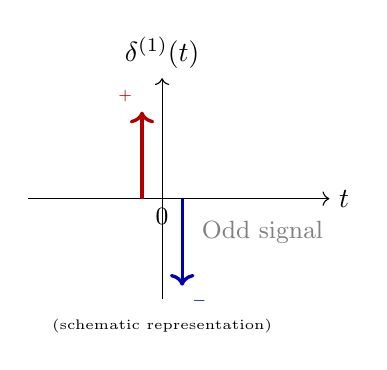
\begin{tikzpicture}[scale=0.85]
  \draw[->] (-2.0,0) -- (2.5,0) node[right] {$t$};
  \draw[->] (0,-1.5) -- (0,1.8) node[above] {$\delta^{(1)}(t)$};
  % Symbolic doublet: positive arrow then negative arrow
  \draw[->, very thick, red!70!black] (-0.3,0) -- (-0.3,1.3);
  \draw[->, very thick, blue!70!black] (0.3,0) -- (0.3,-1.3);
  \node[above left, font=\tiny, red!70!black] at (-0.3,1.3) {$+$};
  \node[below right, font=\tiny, blue!70!black] at (0.3,-1.3) {$-$};
  \node[below, font=\small] at (0,0) {$0$};
  \node[font=\small, color=gray] at (1.5,-0.5) {Odd signal};
  \node[font=\tiny] at (0,-1.9) {(schematic representation)};
\end{tikzpicture}
\end{center}
\end{propbox}

\subsection*{1.5 Summary Table of Impulse Properties}

{\small
\begin{tabular}{@{}llll@{}}
\toprule
\textbf{\#} & \textbf{Property} & \textbf{Formula} & \textbf{Key Remark}\\
\midrule
1 & Unit Area      & $\int_{-\infty}^{\infty}\delta(t)\,dt=1$ & Always holds \\[3pt]
2 & Strength       & $\int A_0\delta(t)\,dt=A_0$ & $A_0$ = weight \\[3pt]
3 & Integration    & $\int_{-\infty}^{t}\delta(\tau)\,d\tau=u(t)$ & Gives step \\[3pt]
4 & Even           & $\delta(-t)=\delta(t)$ & Even symmetry \\[2pt]
5 & Energy/Power   & NENP, $E=P=\infty$ & Not E or P signal \\[2pt]
6 & Time Shift     & $\delta(t)\to\delta(t-t_1)$ & Peak at $t_1$ \\[2pt]
7 & Time Scale     & $\delta(at)=\tfrac{1}{|a|}\delta(t)$ & Scales amplitude \\[3pt]
8 & Multiplication & $x(t)\delta(t-t_1)=x(t_1)\delta(t-t_1)$ & Samples at $t_1$ \\[3pt]
9 & Sifting        & $\int x(t)\delta(t-t_1)\,dt=x(t_1)$ & Extracts value \\[3pt]
10& Derivative     & $\int x(t)\frac{d^n\delta}{dt^n}\,dt=(-1)^n x^{(n)}(t_1)$ & Sign flip per $n$ \\[3pt]
11& Doublet        & $\frac{d}{dt}\delta(t)=\delta^{(1)}(t)$, odd signal & Zero net area \\[2pt]
\bottomrule
\end{tabular}
}

\subsection*{1.6 Solved Problems (Impulse Signal)}

\begin{exbox}
\textbf{i)} $I=\displaystyle\int_{-5}^{4}\delta(t-5)\,dt$:\quad $t_1=5$ is \emph{outside} $[-5,4]$ $\Rightarrow$ $\boxed{I=0}$

\medskip
\textbf{ii)} $I=\displaystyle\int_{-5}^{4}\delta(t-2)\,dt$:\quad $t_1=2$ is \emph{inside} $[-5,4]$ $\Rightarrow$ $\boxed{I=1}$

\medskip
\textbf{iii)} $x(t)=\sin t\cdot\delta(2t-\pi)$:\quad First reduce: $\delta(2t-\pi)=\delta[2(t-\frac{\pi}{2})]=\frac{1}{2}\delta(t-\frac{\pi}{2})$

\hspace{1em}$\Rightarrow x(t)=\sin\!\left(\tfrac{\pi}{2}\right)\cdot\tfrac{1}{2}\delta(t-\tfrac{\pi}{2})=1\cdot\tfrac{1}{2}\delta(t-\tfrac{\pi}{2})=\boxed{\tfrac{1}{2}\delta(t-\tfrac{\pi}{2})}$

\medskip
\textbf{iv)} $I=\displaystyle\int_{-\infty}^{\infty}e^{-2t}\delta(-2t+1)\,dt$:\quad $\delta(-2t+1)=\delta[-2(t-\tfrac{1}{2})]=\tfrac{1}{2}\delta(t-\tfrac{1}{2})$

\hspace{1em}$\Rightarrow I=\tfrac{1}{2}\cdot e^{-2\cdot(1/2)}=\tfrac{1}{2}e^{-1}=\boxed{\dfrac{1}{2e}}$

\medskip
\textbf{v)} $I=\displaystyle\int_{-\infty}^{\infty}\left[\cos\pi t\cdot\delta(t-2)+3\delta(t+1)+\sin\pi t\cdot\delta(2t-1)\right]dt$

\hspace{1em}$I_1=\cos(2\pi)=1$;\quad $I_2=3$;\quad $\delta(2t-1)=\tfrac{1}{2}\delta(t-\tfrac{1}{2})$ so $I_3=\tfrac{1}{2}\sin\!\left(\tfrac{\pi}{2}\right)=\tfrac{1}{2}$

\hspace{1em}$\Rightarrow \boxed{I = 1+3+\tfrac{1}{2}=4.5}$

\medskip
\textbf{vi) [GATE 2016]:} $I=\displaystyle\int_{-\infty}^{\infty}e^{-t}\delta(2t-2)\,dt$:\quad $\delta(2t-2)=\delta[2(t-1)]=\tfrac{1}{2}\delta(t-1)$

\hspace{1em}$\Rightarrow I=\tfrac{1}{2}e^{-1}=\boxed{\dfrac{1}{2e}}$ \quad\textbf{(Ans: a)}

\medskip
\textbf{vii)} $I=\displaystyle\int_{-2}^{2}2t^2\delta(t-4)\,dt$:\quad $t_1=4\notin[-2,2]$ $\Rightarrow I=0$

\hspace{1em}$I=\displaystyle\int_{-10}^{10}2t^2\delta(t-4)\,dt$:\quad $t_1=4\in[-10,10]$ $\Rightarrow I=2(4)^2=2\times16=\boxed{32}$
\end{exbox}

%=============================================================
\section{2.\ Sampling (Sifting) Property of Unit Impulse}
%=============================================================

\subsection*{2.1 Definition}

\begin{defbox}
When $x(t)$ is multiplied by $\delta(t-\tau)$, the impulse \textbf{samples} (picks out) the value of $x$ at exactly $t=\tau$:
\[
x(t)\cdot\delta(t-\tau) = x(\tau)\cdot\delta(t-\tau)
\]
The resulting signal is:
\[
y(t) = x(t)\cdot\delta(t-\tau) = \begin{cases}x(\tau) & t=\tau\\ 0 & t\neq\tau\end{cases}
\]
This is because $\delta(t-\tau)=0$ for all $t\neq\tau$, so the product collapses to a single value $x(\tau)$ at $t=\tau$.
\end{defbox}

\subsection*{2.2 Sifting Integral}

\begin{propbox}
\textbf{Sifting / Sampling Integral:}
\[
\int_{-\infty}^{\infty} x(t)\cdot\delta(t-\tau)\,dt = x(\tau)
\]
\textbf{Proof:}
\begin{enumerate}[noitemsep, topsep=2pt]
  \item Apply multiplication property: $x(t)\delta(t-\tau) = x(\tau)\delta(t-\tau)$
  \item Integrate both sides: $\displaystyle\int_{-\infty}^{\infty}x(t)\delta(t-\tau)\,dt = x(\tau)\displaystyle\int_{-\infty}^{\infty}\delta(t-\tau)\,dt = x(\tau)\cdot 1 = x(\tau)$ \hfill$\square$
\end{enumerate}
This property is fundamental in sampling theory, filter design, and convolution.
\end{propbox}

\begin{center}
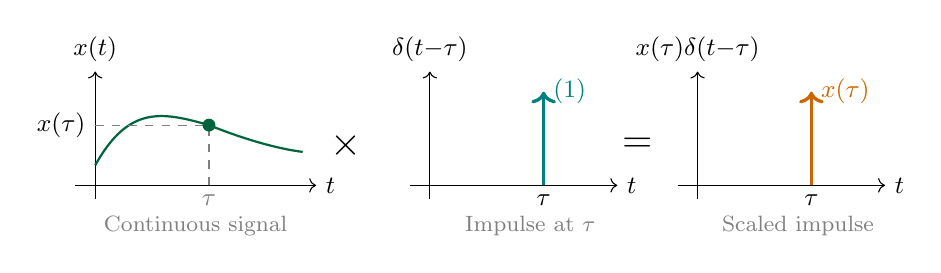
\begin{tikzpicture}[scale=0.85]
  % x(t) panel
  \begin{scope}[xshift=-4.5cm]
    \draw[->](-0.3,0)--(3.3,0) node[right]{\small$t$};
    \draw[->](0,-0.2)--(0,1.7) node[above]{\small$x(t)$};
    \draw[darkgreen,thick](0,0.3)..controls(0.5,1.2)and(1.0,1.1)..(1.7,0.9)
      ..controls(2.2,0.7)and(2.7,0.55)..(3.1,0.5);
    \draw[dashed,gray](1.7,0) node[below]{\small$\tau$}--(1.7,0.9);
    \draw[dashed,gray](0,0.9)--(1.7,0.9);
    \filldraw[darkgreen](1.7,0.9) circle(2.5pt);
    \node[left,font=\small] at(0,0.9){$x(\tau)$};
    \node[font=\footnotesize,color=gray] at(1.5,-0.6){Continuous signal};
  \end{scope}
  \node at(-0.75,0.6){\Large$\times$};
  % delta(t-tau) panel
  \begin{scope}[xshift=0.5cm]
    \draw[->](-0.3,0)--(2.8,0) node[right]{\small$t$};
    \draw[->](0,-0.2)--(0,1.7) node[above]{\small$\delta(t{-}\tau)$};
    \draw[->,very thick,teal](1.7,0)--(1.7,1.4);
    \node[below,font=\small] at(1.7,0){$\tau$};
    \node[right,font=\small,teal] at(1.7,1.4){$(1)$};
    \node[font=\footnotesize,color=gray] at(1.5,-0.6){Impulse at $\tau$};
  \end{scope}
  \node at(3.6,0.6){\Large$=$};
  % result panel
  \begin{scope}[xshift=4.5cm]
    \draw[->](-0.3,0)--(2.8,0) node[right]{\small$t$};
    \draw[->](0,-0.2)--(0,1.7) node[above]{\small$x(\tau)\delta(t{-}\tau)$};
    \draw[->,very thick,orange!80!black](1.7,0)--(1.7,1.4);
    \node[below,font=\small] at(1.7,0){$\tau$};
    \node[right,font=\small,orange!80!black] at(1.7,1.4){$x(\tau)$};
    \node[font=\footnotesize,color=gray] at(1.5,-0.6){Scaled impulse};
  \end{scope}
\end{tikzpicture}
\end{center}

\begin{exbox}
\textbf{Example:} $\delta(t-1)$ samples $x(t)$ at $\tau=1$.
\[
\int_{-\infty}^{\infty}x(t)\cdot\delta(t-1)\,dt = x(1)
\]
If $x(t) = e^{-2t}\cos\pi t$, then $x(1) = e^{-2}\cos\pi = -e^{-2}$.

\medskip
\textbf{General limits:} $\displaystyle\int_{a}^{b} x(t)\,\delta(t-\tau)\,dt = \begin{cases} x(\tau) & a < \tau < b \\ 0 & \tau < a \text{ or } \tau > b \end{cases}$
(boundary at $\tau=a$ or $b$ is conventionally included if using $\geq$)
\end{exbox}

%=============================================================
\section{3.\ Unit Step Signal (Heaviside Step Function)}
%=============================================================

\subsection*{3.1 Definition}

\begin{stepbox}
The \textbf{Unit Step Signal} $u(t)$, also called the \textbf{Heaviside step function}, is:
\[
u(t) = \begin{cases}0 & t < 0\\ 1 & t \geq 0\end{cases}
\quad \text{At } t=0: \text{some conventions define } u(0)=\tfrac{1}{2} \text{ (average); here we use } u(0)=1
\]
It represents switching a signal \textbf{on} at $t=0$. It is used to express causal signals (signals that start at $t=0$).
\end{stepbox}

\begin{center}
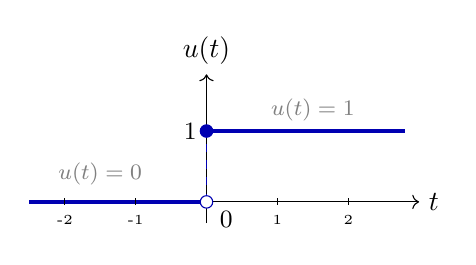
\begin{tikzpicture}[scale=0.9]
  \draw[->](-2.5,0)--(3.0,0) node[right]{$t$};
  \draw[->](0,-0.3)--(0,1.8) node[above]{$u(t)$};
  \draw[blue!70!black,very thick](-2.5,0)--(0,0);
  \draw[blue!70!black,very thick](0,1)--(2.8,1);
  \draw[blue!70!black,dashed](0,0)--(0,1);
  \filldraw[blue!70!black](0,1) circle(2.5pt);
  \filldraw[white,draw=blue!70!black](0,0) circle(2.5pt);
  \node[left,font=\small] at(0,1){$1$};
  \node[below right,font=\small] at(0.05,0){$0$};
  \foreach \x in {-2,-1,1,2}{
    \draw (\x,0.05)--(\x,-0.05) node[below,font=\tiny]{\x};
  }
  \node[font=\footnotesize,color=gray] at(-1.5,0.4){$u(t)=0$};
  \node[font=\footnotesize,color=gray] at(1.5,1.3){$u(t)=1$};
\end{tikzpicture}
\end{center}

\subsection*{3.2 Time-Shifted Unit Step and Signal Windowing}

A shifted step $u(t - t_0)$ turns on at $t = t_0$.  Differences of steps can \emph{gate} (window) other signals:
\[
u(t-a) - u(t-b) = \begin{cases}1 & a \leq t < b \\ 0 & \text{otherwise}\end{cases} \qquad (a < b)
\]

\begin{center}
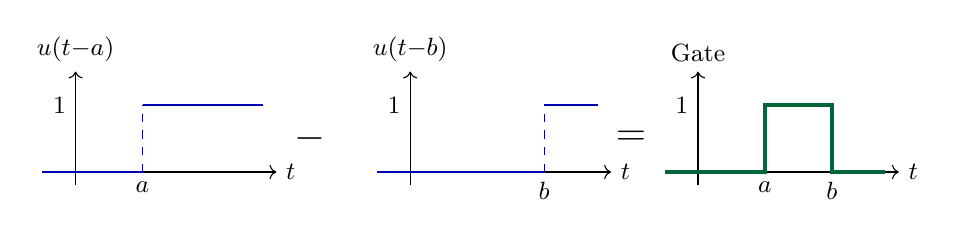
\begin{tikzpicture}[scale=0.85]
  % u(t-a)
  \begin{scope}[xshift=-5cm]
    \draw[->](-0.5,0)--(3.0,0) node[right]{\small$t$};
    \draw[->](0,-0.2)--(0,1.5) node[above]{\small$u(t{-}a)$};
    \draw[blue!70!black,thick](-0.5,0)--(1,0);
    \draw[blue!70!black,thick](1,1)--(2.8,1);
    \draw[blue!70!black,dashed](1,0)--(1,1);
    \node[below,font=\small] at(1,0){$a$};
    \node[left,font=\small] at(0,1){$1$};
  \end{scope}
  \node at(-1.5,0.5){\Large$-$};
  % u(t-b)
  \begin{scope}[xshift=0cm]
    \draw[->](-0.5,0)--(3.0,0) node[right]{\small$t$};
    \draw[->](0,-0.2)--(0,1.5) node[above]{\small$u(t{-}b)$};
    \draw[blue!70!black,thick](-0.5,0)--(2,0);
    \draw[blue!70!black,thick](2,1)--(2.8,1);
    \draw[blue!70!black,dashed](2,0)--(2,1);
    \node[below,font=\small] at(2,0){$b$};
    \node[left,font=\small] at(0,1){$1$};
  \end{scope}
  \node at(3.3,0.5){\Large$=$};
  % result: gate
  \begin{scope}[xshift=4.3cm]
    \draw[->](-0.5,0)--(3.0,0) node[right]{\small$t$};
    \draw[->](0,-0.2)--(0,1.5) node[above]{\small Gate};
    \draw[darkgreen,very thick](-0.5,0)--(1,0)--(1,1)--(2,1)--(2,0)--(2.8,0);
    \node[below,font=\small] at(1,0){$a$};
    \node[below,font=\small] at(2,0){$b$};
    \node[left,font=\small] at(0,1){$1$};
  \end{scope}
\end{tikzpicture}
\end{center}

\subsection*{3.3 Properties of Unit Step Signal}

\begin{propbox}
\textbf{i) Sum $u(t) + u(-t)$:}
\[
u(t) + u(-t) = \begin{cases}1 & t > 0\\ 2 & t = 0\\ 1 & t < 0\end{cases}
\]
For $t>0$: $1+0=1$. For $t<0$: $0+1=1$. At $t=0$: $1+1=2$.

\textbf{Gibbs Phenomenon:} At a discontinuity, averaging the left and right limits gives $\tfrac{0+1}{2}=\tfrac{1}{2}$ (or $\tfrac{1+1}{2}=1$ for $u(t)+u(-t)$, since both sides equal 1 outside $t=0$).

\smallskip
\textbf{ii) Power Calculation:}
\[
P = \lim_{T\to\infty}\frac{1}{2T}\int_{-T}^{T}|u(t)|^2\,dt
= \lim_{T\to\infty}\frac{1}{2T}\left[\int_{-T}^{0}0\,dt+\int_{0}^{T}1\,dt\right]
= \lim_{T\to\infty}\frac{T}{2T} = \frac{1}{2}
\]
$E = \displaystyle\int_0^\infty 1\,dt = \infty$ (infinite energy). $P = \dfrac{1}{2}$ (finite power).

$\Rightarrow$ \textbf{Power signal}. $\quad \text{rms} = \sqrt{P} = \dfrac{1}{\sqrt{2}} \approx 0.707$

\smallskip
\textbf{iii) Symmetry:} $u(t) \neq u(-t)$ and $u(t) \neq -u(-t)$ $\Rightarrow$ \textbf{neither even nor odd}

However, we can decompose $u(t) = u_e(t) + u_o(t)$ where:
\[
u_e(t) = \frac{u(t)+u(-t)}{2} = \frac{1}{2}\quad(t\neq0) \qquad u_o(t) = \frac{u(t)-u(-t)}{2} = \frac{1}{2}\,\text{sgn}(t)
\]

\smallskip
\textbf{iv) Fourier Representation:} The Fourier transform of $u(t)$ involves a delta function at origin:
$U(f) = \frac{1}{2}\delta(f) + \frac{1}{j2\pi f}$ (for reference; covered in Fourier analysis).
\end{propbox}

%=============================================================
\section{4.\ Relation Between Impulse \& Step Signal}
%=============================================================

\subsection*{4.1 Core Relations}

\begin{defbox}
\[
\boxed{\int_{-\infty}^{t}\delta(\tau)\,d\tau = u(t)} \qquad\qquad \boxed{\frac{d\,u(t)}{dt} = \delta(t)}
\]
The \textbf{running integral} of the impulse is the step. The \textbf{derivative} of the step is the impulse.
These are \textbf{dual} relations and among the most important in signals \& systems.
\end{defbox}

\subsection*{4.2 Derivation via the $u_\Delta(t)$ Approximation}

Define a smooth approximation $u_\Delta(t)$ (linear ramp transition over $[0, \Delta]$):
\[
u_\Delta(t) = \begin{cases}0 & t < 0\\ t/\Delta & 0 \leq t \leq \Delta\\ 1 & t > \Delta\end{cases}
\]
Its derivative is:
\[
\frac{d\,u_\Delta(t)}{dt} = \begin{cases}1/\Delta & 0 < t < \Delta\\ 0 & \text{elsewhere}\end{cases}
\quad\Rightarrow\quad \text{Area of derivative} = \Delta \cdot \frac{1}{\Delta} = 1
\]
As $\Delta \to 0$: $u_\Delta(t) \to u(t)$ (step), and $\dfrac{du_\Delta}{dt} \to \delta(t)$ (impulse). This rigorously shows $\dfrac{du}{dt} = \delta(t)$.

\begin{center}
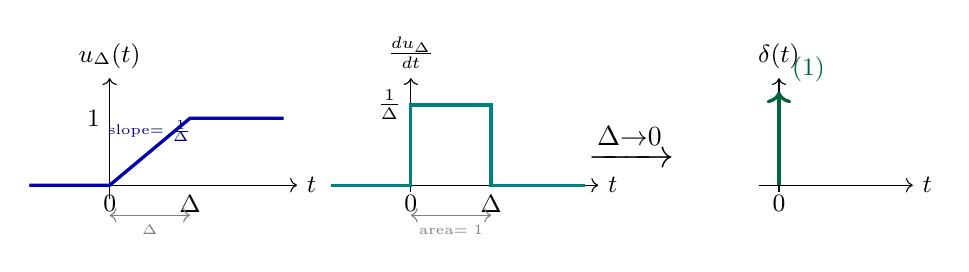
\begin{tikzpicture}[scale=0.85]
  % Left: u_Delta(t)
  \begin{scope}[xshift=-4.5cm]
    \draw[->](-1.2,0)--(2.8,0) node[right]{\small$t$};
    \draw[->](0,-0.2)--(0,1.6) node[above]{\small$u_\Delta(t)$};
    \draw[blue!70!black,very thick](-1.2,0)--(0,0)--(1.2,1)--(2.6,1);
    \node[below,font=\small] at(0,0){$0$};
    \node[below,font=\small] at(1.2,0){$\Delta$};
    \node[left,font=\small] at(0,1){$1$};
    \draw[<->,gray](0,-0.45)--(1.2,-0.45) node[midway,below,font=\tiny]{$\Delta$};
    \node[above,font=\tiny,blue!50!black] at(0.6,0.5){slope$=\tfrac{1}{\Delta}$};
  \end{scope}
  % derivative of u_Delta
  \begin{scope}[xshift=0cm]
    \draw[->](-1.2,0)--(2.8,0) node[right]{\small$t$};
    \draw[->](0,-0.1)--(0,1.6) node[above]{\small$\frac{du_\Delta}{dt}$};
    \draw[teal,very thick](-1.2,0)--(0,0)--(0,1.2)--(1.2,1.2)--(1.2,0)--(2.6,0);
    \node[below,font=\small] at(0,0){$0$};
    \node[below,font=\small] at(1.2,0){$\Delta$};
    \node[left,font=\small] at(0,1.2){$\frac{1}{\Delta}$};
    \draw[<->,gray](0,-0.45)--(1.2,-0.45) node[midway,below,font=\tiny]{area$=1$};
  \end{scope}
  \node at(3.3,0.6){\Large$\xrightarrow{\Delta\to0}$};
  % In the limit
  \begin{scope}[xshift=5.5cm]
    \draw[->](-0.3,0)--(2.0,0) node[right]{\small$t$};
    \draw[->](0,-0.1)--(0,1.6) node[above]{\small$\delta(t)$};
    \draw[->,very thick,darkgreen](0,0)--(0,1.4);
    \node[below,font=\small] at(0,0){$0$};
    \node[above right,font=\small,darkgreen] at(0.05,1.4){$(1)$};
  \end{scope}
\end{tikzpicture}
\end{center}

\subsection*{4.3 Full Signal Chain (Integration \& Differentiation)}

\begin{propbox}
\textbf{Integration Chain:} Each signal is the integral of the one to its left:
\[
\delta(t) \;\xrightarrow{\;I\;}\ u(t) \;\xrightarrow{\;I\;}\ r(t) \;\xrightarrow{\;I\;}\ P(t) \;\xrightarrow{\;I\;}\ \cdots
\]
\textbf{Differentiation Chain:} Each signal is the derivative of the one to its right:
\[
\cdots \;\xrightarrow{\;D\;}\ P(t) \;\xrightarrow{\;D\;}\ r(t) \;\xrightarrow{\;D\;}\ u(t) \;\xrightarrow{\;D\;}\ \delta(t)
\]
\textbf{Key cross-relations:}
\[
\int\!\!\int\delta(t)\,dt^2 = r(t), \qquad \frac{d^2r(t)}{dt^2} = \delta(t), \qquad \frac{d^2P(t)}{dt^2} = u(t)
\]
\end{propbox}

\begin{center}
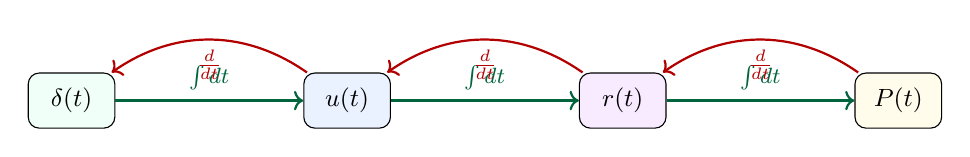
\begin{tikzpicture}[every node/.style={font=\small},scale=1.0]
  \node[draw,rounded corners,fill=lightbg,minimum width=1.1cm,minimum height=0.7cm](d) at(0,0){$\delta(t)$};
  \node[draw,rounded corners,fill=stepbg,minimum width=1.1cm,minimum height=0.7cm](u) at(3.5,0){$u(t)$};
  \node[draw,rounded corners,fill=rampbg,minimum width=1.1cm,minimum height=0.7cm](r) at(7.0,0){$r(t)$};
  \node[draw,rounded corners,fill=expbg,minimum width=1.1cm,minimum height=0.7cm](p) at(10.5,0){$P(t)$};
  \draw[->,thick,darkgreen](d)--node[above,font=\footnotesize]{$\int dt$}(u);
  \draw[->,thick,darkgreen](u)--node[above,font=\footnotesize]{$\int dt$}(r);
  \draw[->,thick,darkgreen](r)--node[above,font=\footnotesize]{$\int dt$}(p);
  \draw[->,thick,red!70!black](p) to[bend right=35] node[below,font=\footnotesize]{$\frac{d}{dt}$}(r);
  \draw[->,thick,red!70!black](r) to[bend right=35] node[below,font=\footnotesize]{$\frac{d}{dt}$}(u);
  \draw[->,thick,red!70!black](u) to[bend right=35] node[below,font=\footnotesize]{$\frac{d}{dt}$}(d);
\end{tikzpicture}
\end{center}

%=============================================================
\section{5.\ Unit Ramp Signal}
%=============================================================

\subsection*{5.1 Definition}

\begin{rampbox}
The \textbf{Unit Ramp signal} is defined as:
\[
r(t) = \begin{cases}0 & t < 0\\ t & t \geq 0\end{cases}
\quad\Leftrightarrow\quad r(t) = t\,u(t)
\]
It is a straight line with \textbf{slope} $m=1$ (a $45^\circ$ line through the origin for $t\geq0$).
The name ``ramp'' comes from its shape resembling an upward incline starting at the origin.
\end{rampbox}

\subsection*{5.2 Graph and Shifted Versions}

\begin{center}
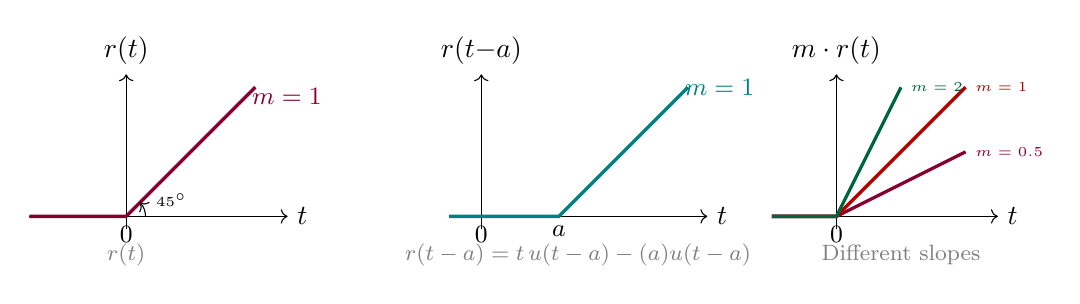
\begin{tikzpicture}[scale=0.82]
  % r(t)
  \begin{scope}[xshift=-5.5cm]
    \draw[->](-1.5,0)--(2.5,0) node[right]{$t$};
    \draw[->](0,-0.2)--(0,2.2) node[above]{$r(t)$};
    \draw[purple!70!black,very thick](-1.5,0)--(0,0)--(2.0,2.0);
    \node[below,font=\small] at(0,0){$0$};
    \node[right,font=\small,purple!70!black] at(1.8,1.85){$m=1$};
    \node[font=\footnotesize,color=gray] at(0,-0.6){$r(t)$};
    \node[font=\tiny] at(0.7,0.25){$45^\circ$};
    % draw 45 degree arc
    \draw[->](0.3,0) arc[start angle=0, end angle=45, radius=0.3];
  \end{scope}
  % r(t - a)
  \begin{scope}[xshift=0cm]
    \draw[->](-0.5,0)--(3.5,0) node[right]{$t$};
    \draw[->](0,-0.2)--(0,2.2) node[above]{$r(t{-}a)$};
    \draw[purple!70!black,very thick,dashed](-0.5,0)--(0,0);
    \draw[teal,very thick](-0.5,0)--(1.2,0)--(3.2,2.0);
    \node[below,font=\small] at(1.2,0){$a$};
    \node[below,font=\small] at(0,0){$0$};
    \node[right,font=\small,teal] at(3.0,2.0){$m=1$};
    \node[font=\footnotesize,color=gray] at(1.5,-0.6){$r(t-a)=t\,u(t-a)-(a)u(t-a)$};
  \end{scope}
  % m*r(t)
  \begin{scope}[xshift=5.5cm]
    \draw[->](-1.0,0)--(2.5,0) node[right]{$t$};
    \draw[->](0,-0.2)--(0,2.2) node[above]{$m\cdot r(t)$};
    \draw[purple!70!black,very thick](-1.0,0)--(0,0)--(2.0,1.0);
    \draw[red!70!black,very thick](-1.0,0)--(0,0)--(2.0,2.0);
    \draw[darkgreen,very thick](-1.0,0)--(0,0)--(1.0,2.0);
    \node[right,font=\tiny,red!70!black] at(2.0,2.0){$m=1$};
    \node[right,font=\tiny,purple!70!black] at(2.0,1.0){$m=0.5$};
    \node[right,font=\tiny,darkgreen] at(1.0,2.0){$m=2$};
    \node[below,font=\small] at(0,0){$0$};
    \node[font=\footnotesize,color=gray] at(1.0,-0.6){Different slopes};
  \end{scope}
\end{tikzpicture}
\end{center}

\subsection*{5.3 Properties of Unit Ramp Signal}

\begin{propbox}
\textbf{i) Integral relation (derives from step):}
\[
r(t) = \int_{-\infty}^{t}u(\tau)\,d\tau = \int_{0}^{t}1\,d\tau = t \quad (t \geq 0)
\]
\[
u(t) \xrightarrow{\int} r(t) \qquad r(t) \xrightarrow{d/dt} u(t)
\]

\textbf{ii) Alternate expressions:}
\[
r(t) = t\,u(t) = \max(t,\, 0) = \frac{t + |t|}{2}
\]

\textbf{iii) Symmetry:} $r(t) \neq r(-t)$ and $r(t) \neq -r(-t)$ $\Rightarrow$ \textbf{neither even nor odd}

Even and odd components:
\[
r_e(t) = \frac{r(t)+r(-t)}{2} = \frac{|t|}{2}, \qquad r_o(t) = \frac{r(t)-r(-t)}{2} = \frac{t}{2}
\]

\textbf{iv) Energy \& Power:}
\[
E = \int_{0}^{\infty}t^2\,dt = \frac{t^3}{3}\bigg|_0^\infty = \infty \qquad P = \lim_{T\to\infty}\frac{1}{2T}\int_{0}^{T}t^2\,dt = \lim_{T\to\infty}\frac{T^2}{6} = \infty
\]
$E = \infty$, $P = \infty$ $\Rightarrow$ \textbf{NENP signal}

\textbf{v) Expressing piecewise linear signals:}
Any piecewise linear (slope-change) waveform can be written as a sum of \emph{ramps} starting at different times with different slopes:
\[
x(t) = m_1\,r(t) + (m_2-m_1)\,r(t-t_1) + (m_3-m_2)\,r(t-t_2) + \cdots
\]
\end{propbox}

%=============================================================
\section{6.\ Unit Parabolic Signal}
%=============================================================

\subsection*{6.1 Definition}

\begin{rampbox}
The \textbf{Unit Parabolic signal} is defined as:
\[
P(t) = \begin{cases}0 & t < 0\\ \dfrac{t^2}{2} & t \geq 0\end{cases}
\quad\Leftrightarrow\quad P(t) = \frac{t^2}{2}\,u(t)
\]
The factor $\tfrac{1}{2}$ ensures $\dfrac{dP}{dt} = t\,u(t) = r(t)$ (i.e., derivative = ramp, not $2t$).
\end{rampbox}

\subsection*{6.2 Graph}

\begin{center}
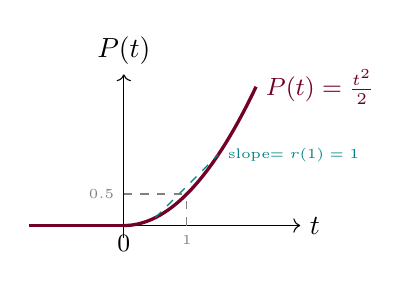
\begin{tikzpicture}[scale=0.80]
  \draw[->](-1.5,0)--(2.8,0) node[right]{$t$};
  \draw[->](0,-0.2)--(0,2.4) node[above]{$P(t)$};
  \draw[purple!60!black,very thick,domain=0:2.1,samples=60] plot(\x,{0.5*\x*\x});
  \draw[purple!60!black,very thick](-1.5,0)--(0,0);
  \node[below,font=\small] at(0,0){$0$};
  \node[right,font=\small,purple!60!black] at(2.1,2.2){$P(t)=\frac{t^2}{2}$};
  % tangent at t=1
  \draw[dashed,teal](0.5,0.125)--(1.5,1.125) node[right,font=\tiny]{slope$=r(1)=1$};
  \draw[dashed,gray](1,0)node[below,font=\tiny]{$1$}--(1,0.5);
  \draw[dashed,gray](0,0.5)node[left,font=\tiny]{$0.5$}--(1,0.5);
\end{tikzpicture}
\end{center}

\subsection*{6.3 Properties}

\begin{propbox}
\textbf{i) Integral Relation:}
\[
P(t) = \int_{-\infty}^{t}r(\tau)\,d\tau = \int_{0}^{t}\tau\,d\tau = \frac{t^2}{2} \quad (t \geq 0)
\qquad \Rightarrow \qquad \frac{dP(t)}{dt} = r(t)
\]

\textbf{ii) Symmetry:} $P(-t) = \frac{t^2}{2}\,u(-t) \neq P(t)$ $\Rightarrow$ \textbf{neither even nor odd}

\textbf{iii) Energy \& Power:}
\[
E = \int_{0}^{\infty}\left(\frac{t^2}{2}\right)^2 dt = \int_{0}^{\infty}\frac{t^4}{4}\,dt = \infty \qquad P = \infty
\]
$E = \infty$, $P = \infty$ $\Rightarrow$ \textbf{NENP signal}

\textbf{iv) Parabola Geometry:}

The relation $2P(t) = t^2$ can be written as $x^2 = 4ay$ with $a = \tfrac{1}{2}$ (here $x \to t$, $y \to P$).
\begin{itemize}
  \item \textbf{Axis of symmetry:} $t = 0$ (the $y$-axis, for $t \geq 0$)
  \item \textbf{Vertex:} $(0, 0)$
  \item \textbf{Focus:} $\left(0, \tfrac{1}{2}\right)$ (at distance $a = \tfrac{1}{2}$ above vertex)
  \item \textbf{Directrix:} $P = -\tfrac{1}{2}$
\end{itemize}
\end{propbox}

\subsection*{6.4 Complete Signal Chain Summary}

\begin{center}
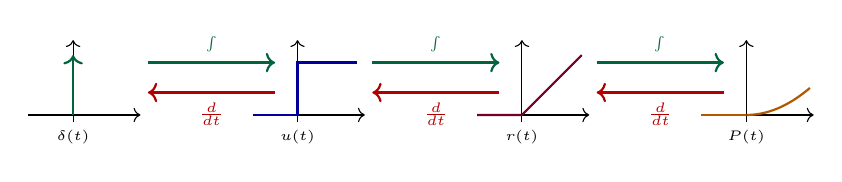
\begin{tikzpicture}[every node/.style={font=\small}, scale=0.95]
  % Draw four waveform mini-plots
  % delta(t)
  \begin{scope}[xshift=0cm,yshift=2.5cm]
    \draw[->](-0.6,0)--(0.9,0); \draw[->](0,-0.1)--(0,1.0);
    \draw[->,thick,darkgreen](0,0)--(0,0.8);
    \node[font=\tiny] at(0,-0.3){$\delta(t)$};
  \end{scope}
  % u(t)
  \begin{scope}[xshift=3cm,yshift=2.5cm]
    \draw[->](-0.6,0)--(0.9,0); \draw[->](0,-0.1)--(0,1.0);
    \draw[blue!60!black,thick](-0.6,0)--(0,0)--(0,0.7)--(0.8,0.7);
    \node[font=\tiny] at(0,-0.3){$u(t)$};
  \end{scope}
  % r(t)
  \begin{scope}[xshift=6cm,yshift=2.5cm]
    \draw[->](-0.6,0)--(0.9,0); \draw[->](0,-0.1)--(0,1.0);
    \draw[purple!60!black,thick](-0.6,0)--(0,0)--(0.8,0.8);
    \node[font=\tiny] at(0,-0.3){$r(t)$};
  \end{scope}
  % P(t)
  \begin{scope}[xshift=9cm,yshift=2.5cm]
    \draw[->](-0.6,0)--(0.9,0); \draw[->](0,-0.1)--(0,1.0);
    \draw[orange!70!black,thick,domain=0:0.85,samples=20] plot(\x,{0.5*\x*\x+0.0});
    \draw[orange!70!black,thick](-0.6,0)--(0,0);
    \node[font=\tiny] at(0,-0.3){$P(t)$};
  \end{scope}
  % Arrows between them
  \draw[->,thick,darkgreen] (1.0,3.2)--(2.7,3.2) node[midway,above,font=\tiny]{$\int$};
  \draw[->,thick,darkgreen] (4.0,3.2)--(5.7,3.2) node[midway,above,font=\tiny]{$\int$};
  \draw[->,thick,darkgreen] (7.0,3.2)--(8.7,3.2) node[midway,above,font=\tiny]{$\int$};
  \draw[->,thick,red!70!black] (8.7,2.8)--(7.0,2.8) node[midway,below,font=\tiny]{$\frac{d}{dt}$};
  \draw[->,thick,red!70!black] (5.7,2.8)--(4.0,2.8) node[midway,below,font=\tiny]{$\frac{d}{dt}$};
  \draw[->,thick,red!70!black] (2.7,2.8)--(1.0,2.8) node[midway,below,font=\tiny]{$\frac{d}{dt}$};
\end{tikzpicture}
\end{center}

%=============================================================
\section{7.\ Signum Function (Sign Function)}
%=============================================================

\subsection*{7.1 Definition}

\begin{signumbox}
\[
\mathrm{sgn}(t) = \begin{cases}-1 & t < 0\\ 0 & t = 0\\ 1 & t > 0\end{cases}
\qquad \text{``Signum'' = Latin for \textbf{sign}}
\]
Alternate form: $\mathrm{sgn}(t) = \dfrac{|t|}{t}\;(t \neq 0)$, undefined at $t=0$ (value is 0 by convention, \emph{not} $\infty$).
\end{signumbox}

\subsection*{7.2 Graph}

\begin{center}
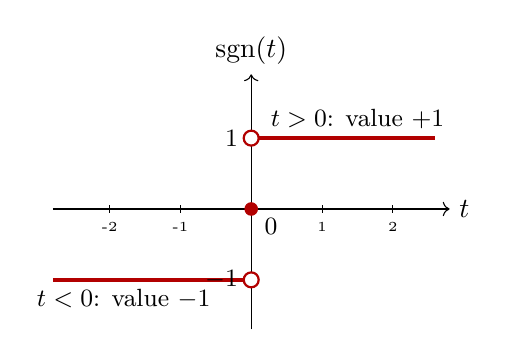
\begin{tikzpicture}[scale=0.9]
  \draw[->](-2.8,0)--(2.8,0) node[right]{$t$};
  \draw[->](0,-1.7)--(0,1.9) node[above]{$\mathrm{sgn}(t)$};
  \draw[red!70!black,very thick](-2.8,-1)--(-0.01,-1);
  \draw[red!70!black,very thick](0.01,1)--(2.6,1);
  \filldraw[white,draw=red!70!black,thick](0,-1) circle(3pt);
  \filldraw[white,draw=red!70!black,thick](0,1) circle(3pt);
  \filldraw[red!70!black](0,0) circle(2.5pt);
  \node[left,font=\small] at(-0.05,1){$1$};
  \node[left,font=\small] at(-0.05,-1){$-1$};
  \node[below right,font=\small] at(0.05,0){$0$};
  \node[below,font=\small] at(-1.8,-1){$t < 0$: value $-1$};
  \node[above,font=\small] at(1.5,1){$t > 0$: value $+1$};
  \foreach \x in {-2,-1,1,2}{
    \draw (\x,0.05)--(\x,-0.05) node[below,font=\tiny]{\x};
  }
\end{tikzpicture}
\end{center}

\subsection*{7.3 Properties of Signum Function}

\begin{propbox}
\textbf{i) Relation to Unit Step:}
\[
1 + \mathrm{sgn}(t) = \begin{cases}0 & t < 0\\ 2 & t > 0\end{cases} = 2\,u(t)
\qquad \Rightarrow \qquad \boxed{\mathrm{sgn}(t) = 2\,u(t) - 1}
\]
This is one of the most important relations. It connects signum directly to the step function.

\begin{center}
\begin{tikzpicture}[scale=0.8]
  \begin{scope}[xshift=-4cm]
    \draw[->](-2,0)--(2.5,0); \draw[->](0,-1.5)--(0,1.5) node[above]{\footnotesize$\mathrm{sgn}(t)$};
    \draw[red!60!black,thick](-2,-1)--(-0.01,-1); \draw[red!60!black,thick](0.01,1)--(2.3,1);
    \filldraw[red!60!black](0,0) circle(2pt);
    \node[left,font=\tiny] at(0,1){$1$}; \node[left,font=\tiny] at(0,-1){$-1$};
  \end{scope}
  \node at(-0.8,0){\small$= 2\,\times$};
  \begin{scope}[xshift=0.8cm]
    \draw[->](-0.5,0)--(2.5,0); \draw[->](0,-0.5)--(0,1.5) node[above]{\footnotesize$u(t)$};
    \draw[blue!60!black,thick](-0.5,0)--(0,0); \draw[blue!60!black,thick](0,1)--(2.3,1);
    \draw[blue!60!black,dashed](0,0)--(0,1);
    \node[left,font=\tiny] at(0,1){$1$};
  \end{scope}
  \node at(3.5,0){\small$-\ 1$};
\end{tikzpicture}
\end{center}

\smallskip
\textbf{ii) Relation to Absolute Value:}
\[
\mathrm{sgn}(t) = \frac{|t|}{t}\;(t\neq0) \qquad \Leftrightarrow \qquad |t| = t\cdot\mathrm{sgn}(t)
\]
\[
\frac{d|t|}{dt} = \mathrm{sgn}(t) \quad (t\neq0) \qquad \Rightarrow \qquad |t| = \int_{-\infty}^{t}\mathrm{sgn}(\tau)\,d\tau + C
\]

\textbf{iii) Derivative --- Relation to Impulse:}

Differentiating $1 + \mathrm{sgn}(t) = 2\,u(t)$ both sides with respect to $t$:
\[
\frac{d}{dt}\mathrm{sgn}(t) = 2\,\frac{d}{dt}u(t) = 2\,\delta(t)
\]
The constant ``1'' on the left vanishes (derivative of a constant = 0).

\textbf{iv) Even/Odd Symmetry:}
\[
\mathrm{sgn}(-t) = -\mathrm{sgn}(t) \qquad \Rightarrow \qquad \textbf{odd function}
\]
This is clear from the graph (point symmetric about origin).

\textbf{v) Energy \& Power:}
\[
E = \int_{-\infty}^{\infty}|\mathrm{sgn}(t)|^2\,dt = \int_{-\infty}^{\infty}1\,dt = \infty
\qquad P = \lim_{T\to\infty}\frac{1}{2T}\int_{-T}^{T}1\,dt = 1
\]
$E = \infty$, $P = 1$ $\Rightarrow$ \textbf{Power signal}. $\quad \text{rms} = \sqrt{1} = 1$.

\textbf{vi) Numerical Examples:}
\[
\mathrm{sgn}(-3) = \frac{3}{-3} = -1 \quad \mathrm{sgn}(7) = 1 \quad \mathrm{sgn}(0) = 0
\]
\textit{HW:} $\mathrm{sgn}(\pi - 3) = ?$ \quad ($\pi \approx 3.14 > 3 \Rightarrow \pi-3 > 0 \Rightarrow$ answer: $\mathbf{1}$)
\end{propbox}

%=============================================================
\section{8.\ Unit Rectangular Function (Gate / Pulse)}
%=============================================================

\subsection*{8.1 Definition}

\begin{rectbox}
The \textbf{Unit Rectangular} (rect) signal is a symmetric pulse of unit area:
\[
\mathrm{rect}(t) = \begin{cases}0 & t < -\dfrac{a}{2}\\ \dfrac{1}{a} & -\dfrac{a}{2} \leq t \leq \dfrac{a}{2}\\ 0 & t > \dfrac{a}{2}\end{cases}
\qquad \text{Area} = a \times \frac{1}{a} = 1 \quad \text{(unit area)}
\]
Also called: \textbf{Unit Rectangular Pulse} or \textbf{Gate function}. Width = $a$, Height = $\tfrac{1}{a}$.
\end{rectbox}

\subsection*{8.2 Graph and Key Parameters}

\begin{center}
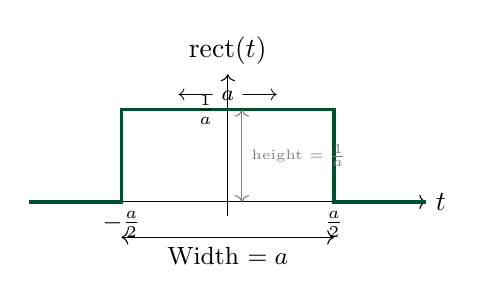
\begin{tikzpicture}[scale=0.90]
  \draw[->](-2.8,0)--(2.8,0) node[right]{$t$};
  \draw[->](0,-0.2)--(0,1.8) node[above]{$\mathrm{rect}(t)$};
  \draw[darkgreen!80!black,very thick](-2.8,0)--(-1.5,0)--(-1.5,1.3)--(1.5,1.3)--(1.5,0)--(2.8,0);
  \node[below,font=\small] at(-1.5,0){$-\frac{a}{2}$};
  \node[below,font=\small] at(1.5,0){$\frac{a}{2}$};
  \node[left,font=\small] at(-0.05,1.3){$\frac{1}{a}$};
  \draw[<->](-1.5,-0.5)--(1.5,-0.5) node[midway,below,font=\small]{Width $= a$};
  % Area annotation
  \draw[<->,gray](0.2,0)--(0.2,1.3) node[midway,right,font=\tiny]{height $=\frac{1}{a}$};
  \node[font=\footnotesize,above] at(0,1.3){$\longleftarrow a \longrightarrow$};
\end{tikzpicture}
\end{center}

\subsection*{8.3 Expression as Difference of Steps}

A rectangular window can be written as the difference of two step functions:
\[
\mathrm{rect}(t) = \frac{1}{a}\left[u\!\left(t + \frac{a}{2}\right) - u\!\left(t - \frac{a}{2}\right)\right]
\]
This allows rectangular pulses to be manipulated algebraically using step function properties.

As $a \to 0$: $\mathrm{rect}(t) \to \delta(t)$ (recovers the impulse with unit area).

\subsection*{8.4 Properties}

\begin{propbox}
\textbf{i) Even Symmetry:} $\mathrm{rect}(-t) = \mathrm{rect}(t)$ $\Rightarrow$ \textbf{even function}

\textbf{ii) Energy:}
\[
E = \int_{-a/2}^{a/2}\left(\frac{1}{a}\right)^2 dt = \frac{1}{a^2} \cdot a = \frac{1}{a} \quad \text{(finite)} \quad \Rightarrow \textbf{ Energy signal}
\]

\textbf{iii) Power:}
\[
P = \lim_{T\to\infty}\frac{1}{2T}\int_{-a/2}^{a/2}\frac{1}{a^2}\,dt = \lim_{T\to\infty}\frac{1}{2T}\cdot\frac{1}{a} = 0
\]
$E = \tfrac{1}{a}$ (finite), $P = 0$ $\Rightarrow$ Confirmed \textbf{Energy signal}.

\textbf{iv) Fourier Transform (for reference):}
\[
\mathcal{F}\{\mathrm{rect}(t/a)\} = a\,\mathrm{sinc}(af) = a\frac{\sin(\pi a f)}{\pi a f}
\]
This shows the fundamental duality: a rectangular pulse in time $\leftrightarrow$ a sinc in frequency.

\textbf{v) As $a \to \infty$:} rect becomes wider and shorter ($\frac{1}{a} \to 0$). At $a=\infty$, rect(t) = 0 everywhere; not a valid signal.
\end{propbox}

%=============================================================
\section{9.\ Unit Triangular Function}
%=============================================================

\subsection*{9.1 Definition}

\begin{rectbox}
The \textbf{Unit Triangular signal} $\mathrm{tri}(t)$ (also $\Lambda(t)$) is a piecewise linear symmetric trianglular pulse:
\[
\mathrm{tri}(t) = \begin{cases}t+1 & -1 \leq t \leq 0\\ -t+1 & 0 \leq t \leq 1\\ 0 & \text{otherwise}\end{cases}
\quad = \max(1-|t|,\; 0) \qquad A = \tfrac{1}{2}\times 2 \times 1 = 1 \text{ (unit area)}
\]
Peak value $= 1$ at $t = 0$. Base extends from $t = -1$ to $t = 1$.
\end{rectbox}

\subsection*{9.2 Graph}

\begin{center}
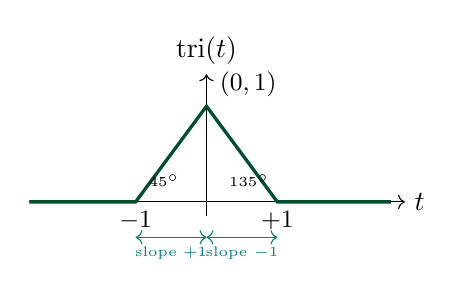
\begin{tikzpicture}[scale=0.90]
  \draw[->](-2.5,0)--(2.8,0) node[right]{$t$};
  \draw[->](0,-0.2)--(0,1.8) node[above]{$\mathrm{tri}(t)$};
  \draw[darkgreen!80!black,very thick](-2.5,0)--(-1,0)--(0,1.35)--(1,0)--(2.6,0);
  \node[below,font=\small] at(-1,0){$-1$};
  \node[below,font=\small] at(1,0){$+1$};
  \node[above right,font=\small] at(0.05,1.35){$(0,1)$};
  % Slope annotations
  \draw[<->,teal] (-1,-0.5)--(0,-0.5) node[midway,below,font=\tiny]{slope $+1$};
  \draw[<->,teal] (0,-0.5)--(1,-0.5) node[midway,below,font=\tiny]{slope $-1$};
  % Angle markers
  \node[font=\tiny] at(-0.6,0.3){$45^\circ$};
  \node[font=\tiny] at(0.6,0.3){$135^\circ$};
\end{tikzpicture}
\end{center}

\subsection*{9.3 Properties}

\begin{propbox}
\textbf{i) Even Symmetry:} $\mathrm{tri}(-t) = \mathrm{tri}(t)$ $\Rightarrow$ \textbf{even function}

\textbf{ii) Relation to Rect (Convolution):}
\[
\mathrm{tri}(t) = \mathrm{rect}(t) * \mathrm{rect}(t) \quad \text{(convolution of two rect pulses)}
\]
This is a fundamental result: convolving a rectangular pulse with itself yields a triangular pulse. Useful in signal processing and Fourier analysis.

\textbf{iii) Energy Computation:}
\[
E = \int_{-1}^{0}(t+1)^2\,dt + \int_{0}^{1}(-t+1)^2\,dt
\]
\[
= \left[\frac{(t+1)^3}{3}\right]_{-1}^{0} + \left[-\frac{(-t+1)^3}{3}\right]_{0}^{1}
= \frac{1}{3} + \frac{1}{3} = \frac{2}{3}
\]
$E = \tfrac{2}{3}$ (finite) $\Rightarrow$ \textbf{Energy signal}.

\textbf{iv) Power:}
\[
P = \lim_{T\to\infty}\frac{E}{2T} = \lim_{T\to\infty}\frac{2/3}{2T} = 0
\]
$P = 0$ (confirms energy signal).

\textbf{v) Fourier Transform:}
\[
\mathcal{F}\{\mathrm{tri}(t)\} = \mathrm{sinc}^2(f) = \left(\frac{\sin(\pi f)}{\pi f}\right)^2
\]
(Follows from convolution theorem: convolution in time $\to$ product in frequency, and $\mathcal{F}\{\mathrm{rect}\} = \mathrm{sinc}$.)
\end{propbox}

%=============================================================
\section{10.\ Sinc Function (Cardinal Sine)}
%=============================================================

\subsection*{10.1 Two Definitions}

\begin{expbox2}
\textbf{1) Unnormalized sinc:}\quad
$\mathrm{sinc}(t) = \begin{cases}1 & t=0\\ \dfrac{\sin t}{t} & t\neq0\end{cases}$
\qquad Zeros at: $t = \pm\pi, \pm 2\pi, \pm 3\pi, \ldots$

\medskip
\textbf{2) Normalized sinc (engineering convention):}\quad
$\mathrm{sinc}(t) = \begin{cases}1 & t=0\\ \dfrac{\sin(\pi t)}{\pi t} & t\neq0\end{cases}$
\qquad Zeros at: $t = \pm 1, \pm 2, \pm 3, \ldots$ (integers)

\medskip
Both forms agree: $\mathrm{sinc}(0) = \lim_{t\to0}\dfrac{\sin(\pi t)}{\pi t} = 1$ (by L'H\^opital's rule or Taylor expansion).
\end{expbox2}

\subsection*{10.2 Graph of Sinc Function}

\begin{center}
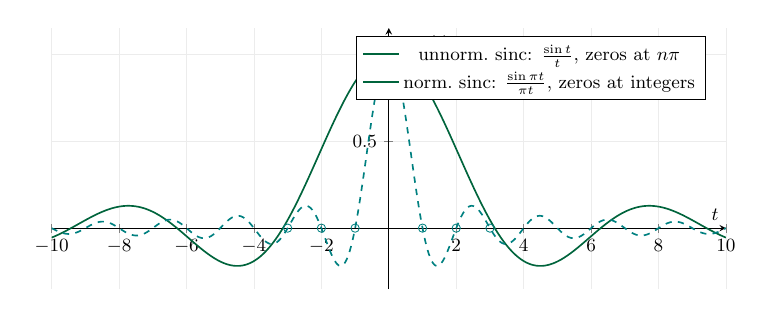
\begin{tikzpicture}[scale=0.75]
  \begin{axis}[
    width=13cm, height=6cm,
    xlabel={$t$}, ylabel={sinc$(t)$},
    xmin=-10, xmax=10, ymin=-0.35, ymax=1.15,
    axis lines=center,
    tick label style={font=\small},
    label style={font=\small},
    samples=300,
    grid=both, grid style={gray!15},
    legend pos=north east,
    legend style={font=\small},
  ]
    % Unnormalized sinc
    \addplot[darkgreen,thick,domain=-10:-0.05]{sin(deg(x))/x};
    \addplot[darkgreen,thick,domain=0.05:10]{sin(deg(x))/x};
    \addplot[darkgreen,thick] coordinates{(0,1)};
    \addlegendentry{unnorm.\ sinc: $\frac{\sin t}{t}$, zeros at $n\pi$};
    % Normalized sinc
    \addplot[teal,thick,dashed,domain=-10:-0.05]{sin(deg(pi*x))/(pi*x)};
    \addplot[teal,thick,dashed,domain=0.05:10]{sin(deg(pi*x))/(pi*x)};
    \addplot[teal,thick] coordinates{(0,1)};
    \addlegendentry{norm.\ sinc: $\frac{\sin\pi t}{\pi t}$, zeros at integers};
    % Mark zeros of normalized sinc
    \foreach \n in {-3,-2,-1,1,2,3}{
      \addplot[teal,only marks,mark=o,mark size=2pt] coordinates{(\n,0)};
    }
  \end{axis}
\end{tikzpicture}
\end{center}

\subsection*{10.3 Properties of Sinc Function}

\begin{propbox}
\textbf{i) Even symmetry:} $\mathrm{sinc}(-t) = \mathrm{sinc}(t)$ $\Rightarrow$ \textbf{even function}

(Since $\sin(-t)/(-t) = \sin(t)/t$.)

\textbf{ii) Energy of unnormalized sinc:}
\[
E = \int_{-\infty}^{\infty}\left(\frac{\sin t}{t}\right)^2 dt = \pi \quad \text{(finite)} \quad \Rightarrow \textbf{ Energy signal}
\]
(Evaluated via Parseval's theorem or contour integration.)

\textbf{iii) Energy of scaled sinc:} For $\mathrm{sinc}(at)$:
\[
E = \frac{\pi}{|a|} \qquad \text{Special case: sinc}(\pi t) \Rightarrow E = \frac{\pi}{\pi} = 1
\]

\textbf{iv) Limiting behavior:}
\[
\lim_{t\to\infty}\mathrm{sinc}(t) = 0 \qquad \text{(decays as } 1/t \text{, after oscillation)}
\]

\textbf{v) Zeros of normalized sinc:} at all nonzero integers: $t = \pm1, \pm2, \pm3, \ldots$

\textbf{vi) Fourier transform pair (fundamental):}
\[
\mathrm{rect}(t) \;\xleftrightarrow{\;\mathcal{F}\;}\; \mathrm{sinc}(f) \qquad \text{i.e., } \mathcal{F}\{\mathrm{rect}(t)\} = \frac{\sin(\pi f)}{\pi f}
\]
This rect-sinc duality is one of the cornerstones of Fourier analysis and communications.

\textbf{vii) Role in sampling theory:} The normalized sinc function is the ideal interpolation kernel in the \textbf{Nyquist--Shannon sampling theorem}: a band-limited signal can be perfectly reconstructed by summing shifted sinc functions weighted by its samples.
\end{propbox}

\begin{center}
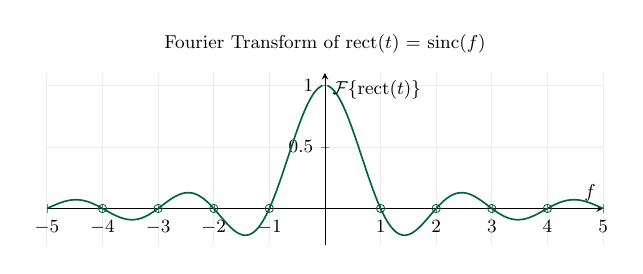
\begin{tikzpicture}[scale=0.75]
  \begin{axis}[
    width=11cm, height=4.5cm,
    xlabel={$f$}, ylabel={$\mathcal{F}\{\mathrm{rect}(t)\}$},
    xmin=-5, xmax=5, ymin=-0.3, ymax=1.1,
    axis lines=center,
    tick label style={font=\small},
    label style={font=\small},
    samples=300,
    grid=both, grid style={gray!15},
    title={Fourier Transform of rect$(t)$ = sinc$(f)$},
    title style={font=\small},
  ]
    \addplot[darkgreen,thick,domain=-5:-0.05]{sin(deg(pi*x))/(pi*x)};
    \addplot[darkgreen,thick,domain=0.05:5]{sin(deg(pi*x))/(pi*x)};
    \addplot[darkgreen,thick] coordinates{(0,1)};
    \foreach \n in {-4,-3,-2,-1,1,2,3,4}{
      \addplot[darkgreen,only marks,mark=o,mark size=2pt] coordinates{(\n,0)};
    }
  \end{axis}
\end{tikzpicture}
\end{center}

%=============================================================
\section{11.\ Exponential Signals (Real \& Complex)}
%=============================================================

\subsection*{11.1 General Form}

\begin{expbox2}
General form: $x(t) = A_0\,e^{\beta t}$ \quad (often set $A_0 = 1$: $x(t) = e^{\beta t}$)

Complex exponent: $\beta = \sigma + j\omega$ \;($\sigma = $ Re part = growth/decay rate, $\omega = $ Im part = oscillation frequency)

\textbf{Euler's formula:} $e^{j\theta} = \cos\theta + j\sin\theta$
\[
x(t) = e^{(\sigma+j\omega)t} = e^{\sigma t} \cdot e^{j\omega t} = e^{\sigma t}(\cos\omega t + j\sin\omega t)
\]
\textbf{Two cases:} (I) $\omega = 0$ (real exponential), (II) $\omega \neq 0$ (complex oscillatory exponential)
\end{expbox2}

\subsection*{11.2 Case I: $\omega = 0$ --- Real Exponential $x(t) = e^{\sigma t}$}

\subsubsection*{Sub-case 1a: $\sigma > 0$ (Growing Exponential)}

\begin{propbox}
$x(t) = e^{\sigma t}$ with $\sigma > 0$: signal grows without bound as $t \to +\infty$.
\begin{itemize}
  \item At $t = 0$: $x(0) = 1$ (all real exponentials start at 1 when $A_0=1$)
  \item Energy: $E = \int_{-\infty}^{\infty}e^{2\sigma t}\,dt = \infty$ (diverges) $\Rightarrow$ NENP signal
  \item Physical examples: population growth, unstable circuit responses, chain reactions
\end{itemize}
\end{propbox}

\subsubsection*{Sub-case 1b: $\sigma < 0$ (Decaying Exponential)}

\begin{propbox}
$x(t) = e^{\sigma t}$ with $\sigma < 0$: signal decays exponentially toward 0.
\begin{itemize}
  \item At $t = 0$: $x(0) = 1$. As $t \to \infty$: $x \to 0$. As $t \to -\infty$: $x \to \infty$.
  \item \textbf{Time constant} $\tau = \frac{1}{|\sigma|}$: time for signal to fall to $e^{-1} \approx 36.8\%$ of initial value.
  \item For causal form $x(t) = e^{\sigma t}u(t)$ ($\sigma < 0$): $E = \int_0^\infty e^{2\sigma t}dt = \frac{1}{2|\sigma|}$ (finite) $\Rightarrow$ Energy signal
  \item Physical examples: RC circuit discharge, radioactive decay, damped spring response
\end{itemize}
\end{propbox}

\subsubsection*{Sub-case 1c: $\sigma = 0$ (DC / Constant Signal)}

$x(t) = e^0 = 1$ for all $t$. Power signal with $P = 1$, $E = \infty$.

\begin{center}
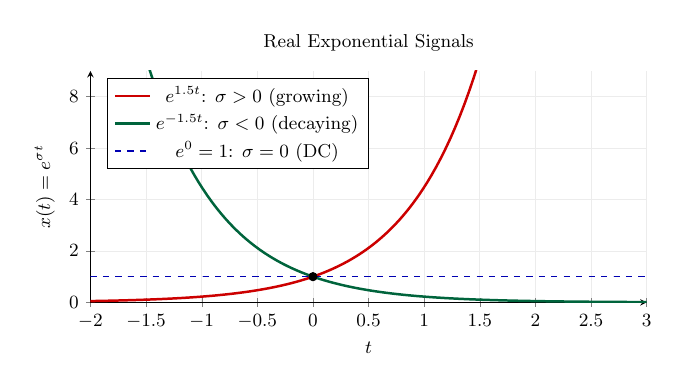
\begin{tikzpicture}[scale=0.75]
  \begin{axis}[
    width=11cm, height=5.5cm,
    xlabel={$t$}, ylabel={$x(t) = e^{\sigma t}$},
    xmin=-2, xmax=3, ymin=0, ymax=9,
    axis lines=left,
    tick label style={font=\small},
    label style={font=\small},
    samples=120, legend pos=north west,
    legend style={font=\small},
    grid=both, grid style={gray!15},
    title={Real Exponential Signals},
    title style={font=\small},
  ]
    \addplot[red!80!black,very thick,domain=-2:3]{exp(1.5*x)};
    \addlegendentry{$e^{1.5t}$: $\sigma>0$ (growing)};
    \addplot[darkgreen,very thick,domain=-2:3]{exp(-1.5*x)};
    \addlegendentry{$e^{-1.5t}$: $\sigma<0$ (decaying)};
    \addplot[blue!70!black,thick,dashed,domain=-2:3]{1};
    \addlegendentry{$e^{0}=1$: $\sigma=0$ (DC)};
    \addplot[mark=*,only marks] coordinates{(0,1)};
  \end{axis}
\end{tikzpicture}
\end{center}

\subsection*{11.3 Case II: $\omega \neq 0$ --- Complex Exponential Signal}

The general complex exponential is:
\[
x(t) = e^{(\sigma+j\omega)t} = e^{\sigma t}(\cos\omega t + j\sin\omega t)
\]
\[
\text{Re}[x(t)] = e^{\sigma t}\cos\omega t \qquad \text{Im}[x(t)] = e^{\sigma t}\sin\omega t
\]

The \textbf{envelope} (instantaneous amplitude) is $|x(t)| = e^{\sigma t}$, which governs growth/decay.

\subsubsection*{Sub-case 2a: $\sigma = 0$ --- Pure Sinusoidal (Constant Envelope)}

\begin{propbox}
$x(t) = e^{j\omega t} = \cos\omega t + j\sin\omega t$

\begin{itemize}
  \item Constant amplitude envelope: $|x(t)| = 1$ for all $t$
  \item Real part: pure cosine. Imaginary part: pure sine.
  \item In 3D: traces a \textbf{helix} on the cylinder of radius 1 (time axis = $t$).
  \item Power signal: $P = 1$, $E = \infty$
  \item This is the fundamental building block of Fourier series and transform.
\end{itemize}
\end{propbox}

\begin{center}
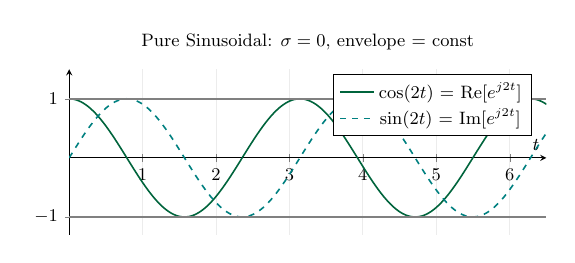
\begin{tikzpicture}[scale=0.72]
  \begin{axis}[
    width=10cm, height=4.5cm,
    xlabel={$t$}, ylabel={},
    xmin=0, xmax=6.5, ymin=-1.3, ymax=1.5,
    axis lines=center,
    tick label style={font=\small},
    label style={font=\small},
    samples=200, legend pos=north east,
    legend style={font=\small},
    grid=both, grid style={gray!15},
    title={Pure Sinusoidal: $\sigma=0$, envelope $=$ const},
    title style={font=\small},
  ]
    \addplot[darkgreen,thick,domain=0:6.5]{cos(deg(2*x))};
    \addlegendentry{$\cos(2t)$ = Re$[e^{j2t}]$};
    \addplot[teal,thick,dashed,domain=0:6.5]{sin(deg(2*x))};
    \addlegendentry{$\sin(2t)$ = Im$[e^{j2t}]$};
    \addplot[gray,thick,domain=0:6.5]{1}; \addplot[gray,thick,domain=0:6.5]{-1};
  \end{axis}
\end{tikzpicture}
\end{center}

\subsubsection*{Sub-case 2b: $\sigma > 0$ --- Growing Oscillation (Diverging Envelope)}

\begin{propbox}
$x(t) = e^{(\sigma+j\omega)t}$ with $\sigma > 0$:
\[
\text{Re}[x(t)] = e^{\sigma t}\cos\omega t \qquad \text{Im}[x(t)] = e^{\sigma t}\sin\omega t
\]
\begin{itemize}
  \item Envelope $= e^{\sigma t}$ grows exponentially $\to$ oscillations increase in amplitude
  \item Signal is \textbf{unstable}: energy $\to \infty$; NENP signal
  \item Physical examples: unstable feedback systems, parametric oscillation
\end{itemize}
\end{propbox}

\begin{center}
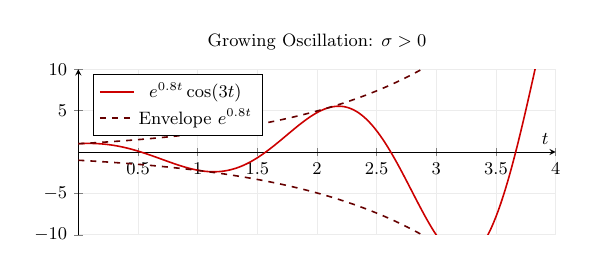
\begin{tikzpicture}[scale=0.72]
  \begin{axis}[
    width=10cm, height=4.5cm,
    xlabel={$t$}, ylabel={},
    xmin=0, xmax=4, ymin=-10, ymax=10,
    axis lines=center,
    tick label style={font=\small},
    label style={font=\small},
    samples=200, legend pos=north west,
    legend style={font=\small},
    grid=both, grid style={gray!15},
    title={Growing Oscillation: $\sigma>0$},
    title style={font=\small},
  ]
    \addplot[red!80!black,thick,domain=0:4]{exp(0.8*x)*cos(deg(3*x))};
    \addlegendentry{$e^{0.8t}\cos(3t)$};
    \addplot[red!40!black,dashed,thick,domain=0:4]{exp(0.8*x)};
    \addlegendentry{Envelope $e^{0.8t}$};
    \addplot[red!40!black,dashed,thick,domain=0:4]{-exp(0.8*x)};
  \end{axis}
\end{tikzpicture}
\end{center}

\subsubsection*{Sub-case 2c: $\sigma < 0$ --- Damped Oscillation (Decaying Envelope)}

\begin{propbox}
$x(t) = e^{(\sigma+j\omega)t}$ with $\sigma < 0$:
\[
\text{Re}[x(t)] = e^{\sigma t}\cos\omega t \qquad \text{Im}[x(t)] = e^{\sigma t}\sin\omega t
\]
\begin{itemize}
  \item Envelope $= e^{\sigma t}$ decays exponentially $\to$ oscillations diminish and $\to 0$
  \item Signal is \textbf{stable}: energy is finite for causal version $\Rightarrow$ Energy signal
  \item Physical examples: \textbf{RLC circuit} transient response, damped mechanical vibration, audio decay
  \item The \textbf{time constant} $\tau = 1/|\sigma|$ controls how fast the oscillation dies out
\end{itemize}
\end{propbox}

\begin{center}
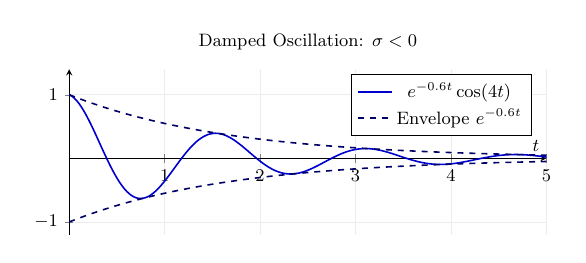
\begin{tikzpicture}[scale=0.72]
  \begin{axis}[
    width=10cm, height=4.5cm,
    xlabel={$t$}, ylabel={},
    xmin=0, xmax=5, ymin=-1.2, ymax=1.4,
    axis lines=center,
    tick label style={font=\small},
    label style={font=\small},
    samples=200, legend pos=north east,
    legend style={font=\small},
    grid=both, grid style={gray!15},
    title={Damped Oscillation: $\sigma<0$},
    title style={font=\small},
  ]
    \addplot[blue!80!black,thick,domain=0:5]{exp(-0.6*x)*cos(deg(4*x))};
    \addlegendentry{$e^{-0.6t}\cos(4t)$};
    \addplot[blue!40!black,dashed,thick,domain=0:5]{exp(-0.6*x)};
    \addlegendentry{Envelope $e^{-0.6t}$};
    \addplot[blue!40!black,dashed,thick,domain=0:5]{-exp(-0.6*x)};
  \end{axis}
\end{tikzpicture}
\end{center}

\subsection*{11.4 Summary: All Cases of Complex Exponential $e^{(\sigma+j\omega)t}$}

\begin{center}
{\small
\begin{tabular}{@{}cclll@{}}
\toprule
\textbf{$\sigma$} & \textbf{$\omega$} & \textbf{Type} & \textbf{Behavior} & \textbf{Signal Class}\\
\midrule
$> 0$ & $0$        & Real growing        & Monotone increase $\to\infty$    & NENP\\
$= 0$ & $0$        & DC (constant)       & Flat line $= 1$                  & Power ($P=1$)\\
$< 0$ & $0$        & Real decaying       & Monotone decrease $\to 0$        & NENP (or E if causal)\\
$= 0$ & $\neq 0$   & Pure sinusoid       & Constant-amplitude oscillation   & Power ($P=\frac{1}{2}$)\\
$> 0$ & $\neq 0$   & Growing oscillation & Expanding-amplitude oscillation  & NENP\\
$< 0$ & $\neq 0$   & Damped oscillation  & Decaying-amplitude oscillation   & E signal (if causal)\\
\bottomrule
\end{tabular}
}
\end{center}

\subsection*{11.5 Euler's Formula and Sinusoidal Decomposition}

From Euler's formula, sinusoids can be expressed using complex exponentials:
\[
\cos\omega t = \frac{e^{j\omega t} + e^{-j\omega t}}{2} \qquad \sin\omega t = \frac{e^{j\omega t} - e^{-j\omega t}}{2j}
\]
This decomposition is fundamental to Fourier analysis, phasor representation, and filter theory.

\begin{center}
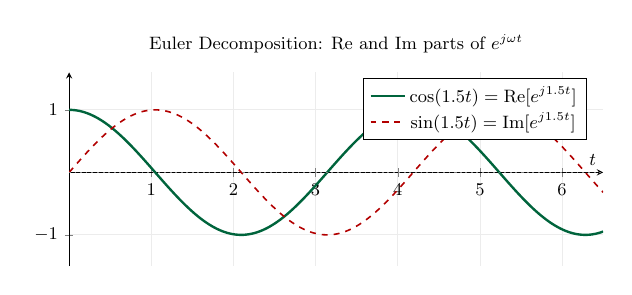
\begin{tikzpicture}[scale=0.72]
  \begin{axis}[
    width=11cm, height=5.0cm,
    xlabel={$t$}, ylabel={},
    xmin=0, xmax=6.5, ymin=-1.5, ymax=1.6,
    axis lines=center,
    tick label style={font=\small},
    label style={font=\small},
    samples=200, legend pos=north east,
    legend style={font=\small},
    grid=both, grid style={gray!15},
    title={Euler Decomposition: Re and Im parts of $e^{j\omega t}$},
    title style={font=\small},
  ]
    \addplot[darkgreen,very thick,domain=0:6.5]{cos(deg(1.5*x))};
    \addlegendentry{$\cos(1.5t)=\mathrm{Re}[e^{j1.5t}]$};
    \addplot[red!70!black,thick,dashed,domain=0:6.5]{sin(deg(1.5*x))};
    \addlegendentry{$\sin(1.5t)=\mathrm{Im}[e^{j1.5t}]$};
    \addplot[gray,thick,dotted,domain=0:6.5]{0};
  \end{axis}
\end{tikzpicture}
\end{center}

\vspace{8pt}

\begin{propbox}
\textbf{Complete Signal Classification Summary:}

{\small
\begin{tabular}{@{}llccc@{}}
\toprule
\textbf{Signal} & \textbf{Formula} & \textbf{Even/Odd} & \textbf{E/P Class} & \textbf{Value at $t=0$}\\
\midrule
Impulse $\delta(t)$     & $\infty$ at $t=0$, else 0          & Even    & NENP        & $\infty$\\
Step $u(t)$             & 0 for $t<0$, 1 for $t\geq0$        & Neither & Power ($\frac{1}{2}$) & 1\\
Ramp $r(t)$             & $t\,u(t)$                           & Neither & NENP        & 0\\
Parabolic $P(t)$        & $\frac{t^2}{2}\,u(t)$               & Neither & NENP        & 0\\
Signum sgn$(t)$         & $\pm1$ or 0                         & Odd     & Power (1)   & 0\\
Rectangular rect$(t)$   & $\frac{1}{a}$ over $|t|\leq\frac{a}{2}$ & Even & Energy ($\frac{1}{a}$) & $\frac{1}{a}$\\
Triangular tri$(t)$     & $1-|t|$ over $|t|\leq1$             & Even    & Energy ($\frac{2}{3}$) & 1\\
Sinc sinc$(t)$          & $\frac{\sin t}{t}$                  & Even    & Energy ($\pi$) & 1\\
Exp (growing) $e^{\sigma t}$ ($\sigma>0$) & monotone $\uparrow$ & Neither & NENP & 1\\
Exp (decaying) $e^{\sigma t}u(t)$ ($\sigma<0$) & decays to 0  & Neither & Energy & 1\\
Pure sinusoid $\cos\omega t$ & oscillates $\pm1$               & Even    & Power ($\frac{1}{2}$) & 1\\
\bottomrule
\end{tabular}
}
\end{propbox}

\vspace{6pt}
\begin{center}
\small\color{gray}
Signals \& Systems $\cdot$ Comprehensive Reference $\cdot$ Elementary Signals (Impulse through Exponential)\\
\textit{Topics: Unit Impulse, Sampling Property, Unit Step, Impulse-Step Relation, Ramp, Parabolic, Signum, Rect, Tri, Sinc, Exponential}
\end{center}

\end{document}